\documentclass[twoside]{book}

% Packages required by doxygen
\usepackage{fixltx2e}
\usepackage{calc}
\usepackage{doxygen}
\usepackage[export]{adjustbox} % also loads graphicx
\usepackage{graphicx}
\usepackage[utf8]{inputenc}
\usepackage{makeidx}
\usepackage{multicol}
\usepackage{multirow}
\PassOptionsToPackage{warn}{textcomp}
\usepackage{textcomp}
\usepackage[nointegrals]{wasysym}
\usepackage[table]{xcolor}

% Font selection
\usepackage[T1]{fontenc}
\usepackage[scaled=.90]{helvet}
\usepackage{courier}
\usepackage{amssymb}
\usepackage{sectsty}
\renewcommand{\familydefault}{\sfdefault}
\allsectionsfont{%
  \fontseries{bc}\selectfont%
  \color{darkgray}%
}
\renewcommand{\DoxyLabelFont}{%
  \fontseries{bc}\selectfont%
  \color{darkgray}%
}
\newcommand{\+}{\discretionary{\mbox{\scriptsize$\hookleftarrow$}}{}{}}

% Page & text layout
\usepackage{geometry}
\geometry{%
  a4paper,%
  top=2.5cm,%
  bottom=2.5cm,%
  left=2.5cm,%
  right=2.5cm%
}
\tolerance=750
\hfuzz=15pt
\hbadness=750
\setlength{\emergencystretch}{15pt}
\setlength{\parindent}{0cm}
\setlength{\parskip}{3ex plus 2ex minus 2ex}
\makeatletter
\renewcommand{\paragraph}{%
  \@startsection{paragraph}{4}{0ex}{-1.0ex}{1.0ex}{%
    \normalfont\normalsize\bfseries\SS@parafont%
  }%
}
\renewcommand{\subparagraph}{%
  \@startsection{subparagraph}{5}{0ex}{-1.0ex}{1.0ex}{%
    \normalfont\normalsize\bfseries\SS@subparafont%
  }%
}
\makeatother

% Headers & footers
\usepackage{fancyhdr}
\pagestyle{fancyplain}
\fancyhead[LE]{\fancyplain{}{\bfseries\thepage}}
\fancyhead[CE]{\fancyplain{}{}}
\fancyhead[RE]{\fancyplain{}{\bfseries\leftmark}}
\fancyhead[LO]{\fancyplain{}{\bfseries\rightmark}}
\fancyhead[CO]{\fancyplain{}{}}
\fancyhead[RO]{\fancyplain{}{\bfseries\thepage}}
\fancyfoot[LE]{\fancyplain{}{}}
\fancyfoot[CE]{\fancyplain{}{}}
\fancyfoot[RE]{\fancyplain{}{\bfseries\scriptsize Generated by Doxygen }}
\fancyfoot[LO]{\fancyplain{}{\bfseries\scriptsize Generated by Doxygen }}
\fancyfoot[CO]{\fancyplain{}{}}
\fancyfoot[RO]{\fancyplain{}{}}
\renewcommand{\footrulewidth}{0.4pt}
\renewcommand{\chaptermark}[1]{%
  \markboth{#1}{}%
}
\renewcommand{\sectionmark}[1]{%
  \markright{\thesection\ #1}%
}

% Indices & bibliography
\usepackage{natbib}
\usepackage[titles]{tocloft}
\setcounter{tocdepth}{3}
\setcounter{secnumdepth}{5}
\makeindex

% Hyperlinks (required, but should be loaded last)
\usepackage{ifpdf}
\ifpdf
  \usepackage[pdftex,pagebackref=true]{hyperref}
\else
  \usepackage[ps2pdf,pagebackref=true]{hyperref}
\fi
\hypersetup{%
  colorlinks=true,%
  linkcolor=blue,%
  citecolor=blue,%
  unicode%
}

% Custom commands
\newcommand{\clearemptydoublepage}{%
  \newpage{\pagestyle{empty}\cleardoublepage}%
}

\usepackage{caption}
\captionsetup{labelsep=space,justification=centering,font={bf},singlelinecheck=off,skip=4pt,position=top}

%===== C O N T E N T S =====

\begin{document}

% Titlepage & ToC
\hypersetup{pageanchor=false,
             bookmarksnumbered=true,
             pdfencoding=unicode
            }
\pagenumbering{alph}
\begin{titlepage}
\vspace*{7cm}
\begin{center}%
{\Large Atlantik \\[1ex]\large 1.\+1.\+0 }\\
\vspace*{1cm}
{\large Generated by Doxygen 1.8.13}\\
\end{center}
\end{titlepage}
\clearemptydoublepage
\pagenumbering{roman}
\tableofcontents
\clearemptydoublepage
\pagenumbering{arabic}
\hypersetup{pageanchor=true}

%--- Begin generated contents ---
\chapter{Hierarchical Index}
\section{Class Hierarchy}
This inheritance list is sorted roughly, but not completely, alphabetically\+:\begin{DoxyCompactList}
\item \contentsline{section}{Bateau}{\pageref{class_bateau}}{}
\begin{DoxyCompactList}
\item \contentsline{section}{Bateau\+Voyageur}{\pageref{class_bateau_voyageur}}{}
\end{DoxyCompactList}
\item \contentsline{section}{Equipement}{\pageref{class_equipement}}{}
\item \contentsline{section}{Passerelle}{\pageref{class_passerelle}}{}
\item Q\+Sql\+Query\begin{DoxyCompactList}
\item \contentsline{section}{jeu\+Enregistrement}{\pageref{classjeu_enregistrement}}{}
\end{DoxyCompactList}
\item Q\+Text\+Document\begin{DoxyCompactList}
\item \contentsline{section}{P\+DF}{\pageref{class_p_d_f}}{}
\end{DoxyCompactList}
\end{DoxyCompactList}

\chapter{Class Index}
\section{Class List}
Here are the classes, structs, unions and interfaces with brief descriptions\+:\begin{DoxyCompactList}
\item\contentsline{section}{\hyperlink{class_bateau}{Bateau} }{\pageref{class_bateau}}{}
\item\contentsline{section}{\hyperlink{class_bateau_voyageur}{Bateau\+Voyageur} }{\pageref{class_bateau_voyageur}}{}
\item\contentsline{section}{\hyperlink{class_equipement}{Equipement} }{\pageref{class_equipement}}{}
\item\contentsline{section}{\hyperlink{classjeu_enregistrement}{jeu\+Enregistrement} }{\pageref{classjeu_enregistrement}}{}
\item\contentsline{section}{\hyperlink{class_passerelle}{Passerelle} }{\pageref{class_passerelle}}{}
\item\contentsline{section}{\hyperlink{class_p_d_f}{P\+DF} }{\pageref{class_p_d_f}}{}
\end{DoxyCompactList}

\chapter{Class Documentation}
\hypertarget{class_bateau}{}\section{Bateau Class Reference}
\label{class_bateau}\index{Bateau@{Bateau}}


Inheritance diagram for Bateau\+:\nopagebreak
\begin{figure}[H]
\begin{center}
\leavevmode
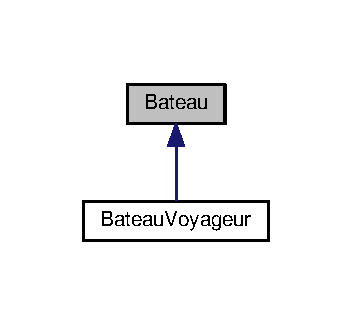
\includegraphics[width=169pt]{class_bateau__inherit__graph}
\end{center}
\end{figure}
\subsection*{Public Member Functions}
\begin{DoxyCompactItemize}
\item 
\mbox{\Hypertarget{class_bateau_a5ea29ce02b632a199385200248a05581}\label{class_bateau_a5ea29ce02b632a199385200248a05581}} 
{\bfseries Bateau} (Q\+String un\+Id, Q\+String un\+Nom, float une\+Longueur, float une\+Largeur)
\item 
Q\+String \hyperlink{class_bateau_a392f6a45649a2a35186dfcd1ca58eddc}{vers\+Chaine} ()
\begin{DoxyCompactList}\small\item\em \hyperlink{class_bateau_a392f6a45649a2a35186dfcd1ca58eddc}{Bateau\+::vers\+Chaine}. \end{DoxyCompactList}\end{DoxyCompactItemize}


\subsection{Member Function Documentation}
\mbox{\Hypertarget{class_bateau_a392f6a45649a2a35186dfcd1ca58eddc}\label{class_bateau_a392f6a45649a2a35186dfcd1ca58eddc}} 
\index{Bateau@{Bateau}!vers\+Chaine@{vers\+Chaine}}
\index{vers\+Chaine@{vers\+Chaine}!Bateau@{Bateau}}
\subsubsection{\texorpdfstring{vers\+Chaine()}{versChaine()}}
{\footnotesize\ttfamily Q\+String Bateau\+::vers\+Chaine (\begin{DoxyParamCaption}{ }\end{DoxyParamCaption})}



\hyperlink{class_bateau_a392f6a45649a2a35186dfcd1ca58eddc}{Bateau\+::vers\+Chaine}. 

\begin{DoxyReturn}{Returns}
chaine avec infos principal des bateaux. Retourne sous la forme d\textquotesingle{}une chaîne de caractères toutes les valeurs des attributs de la classe et de leur libellés 
\end{DoxyReturn}


The documentation for this class was generated from the following files\+:\begin{DoxyCompactItemize}
\item 
/home/jeremy/\+Documents/qt\+Creator/\+Generation\+P\+D\+F\+\_\+\+Atlantik/bateau.\+h\item 
/home/jeremy/\+Documents/qt\+Creator/\+Generation\+P\+D\+F\+\_\+\+Atlantik/bateau.\+cpp\end{DoxyCompactItemize}

\hypertarget{class_bateau_voyageur}{}\section{Bateau\+Voyageur Class Reference}
\label{class_bateau_voyageur}\index{Bateau\+Voyageur@{Bateau\+Voyageur}}


Inheritance diagram for Bateau\+Voyageur\+:\nopagebreak
\begin{figure}[H]
\begin{center}
\leavevmode
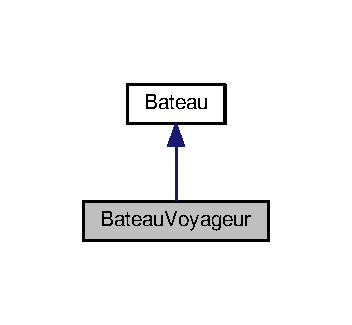
\includegraphics[width=169pt]{class_bateau_voyageur__inherit__graph}
\end{center}
\end{figure}


Collaboration diagram for Bateau\+Voyageur\+:\nopagebreak
\begin{figure}[H]
\begin{center}
\leavevmode
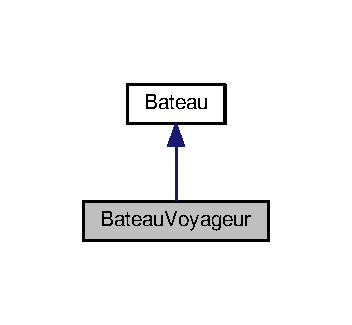
\includegraphics[width=169pt]{class_bateau_voyageur__coll__graph}
\end{center}
\end{figure}
\subsection*{Public Member Functions}
\begin{DoxyCompactItemize}
\item 
\hyperlink{class_bateau_voyageur_ac327b0101a2586190a3afcd639f146cc}{Bateau\+Voyageur} ()
\item 
\hyperlink{class_bateau_voyageur_ad23d17c60d5aaa25ae2a1304782aae4c}{Bateau\+Voyageur} (Q\+String un\+Id, Q\+String un\+Nom, float une\+Longueur, float une\+Largeur, float vitesse, Q\+String une\+Image, Q\+Vector$<$ \hyperlink{class_equipement}{Equipement} $>$ un\+Vect\+Equip)
\begin{DoxyCompactList}\small\item\em \hyperlink{class_bateau_voyageur_ac327b0101a2586190a3afcd639f146cc}{Bateau\+Voyageur\+::\+Bateau\+Voyageur}. \end{DoxyCompactList}\item 
Q\+String \hyperlink{class_bateau_voyageur_a3fa14cf7db3a1a35457f1e0450d7e8b2}{vers\+Chaine} ()
\begin{DoxyCompactList}\small\item\em \hyperlink{class_bateau_voyageur_a3fa14cf7db3a1a35457f1e0450d7e8b2}{Bateau\+Voyageur\+::vers\+Chaine}. \end{DoxyCompactList}\item 
Q\+String \hyperlink{class_bateau_voyageur_a3154786b2f572d0c2a2ac975757295eb}{get\+Image\+Bat\+Voy} ()
\begin{DoxyCompactList}\small\item\em \hyperlink{class_bateau_voyageur_a3154786b2f572d0c2a2ac975757295eb}{Bateau\+Voyageur\+::get\+Image\+Bat\+Voy}. \end{DoxyCompactList}\end{DoxyCompactItemize}


\subsection{Constructor \& Destructor Documentation}
\mbox{\Hypertarget{class_bateau_voyageur_ac327b0101a2586190a3afcd639f146cc}\label{class_bateau_voyageur_ac327b0101a2586190a3afcd639f146cc}} 
\index{Bateau\+Voyageur@{Bateau\+Voyageur}!Bateau\+Voyageur@{Bateau\+Voyageur}}
\index{Bateau\+Voyageur@{Bateau\+Voyageur}!Bateau\+Voyageur@{Bateau\+Voyageur}}
\subsubsection{\texorpdfstring{Bateau\+Voyageur()}{BateauVoyageur()}\hspace{0.1cm}{\footnotesize\ttfamily [1/2]}}
{\footnotesize\ttfamily Bateau\+Voyageur\+::\+Bateau\+Voyageur (\begin{DoxyParamCaption}{ }\end{DoxyParamCaption})}

Class Héritante de \hyperlink{class_bateau}{Bateau} \mbox{\Hypertarget{class_bateau_voyageur_ad23d17c60d5aaa25ae2a1304782aae4c}\label{class_bateau_voyageur_ad23d17c60d5aaa25ae2a1304782aae4c}} 
\index{Bateau\+Voyageur@{Bateau\+Voyageur}!Bateau\+Voyageur@{Bateau\+Voyageur}}
\index{Bateau\+Voyageur@{Bateau\+Voyageur}!Bateau\+Voyageur@{Bateau\+Voyageur}}
\subsubsection{\texorpdfstring{Bateau\+Voyageur()}{BateauVoyageur()}\hspace{0.1cm}{\footnotesize\ttfamily [2/2]}}
{\footnotesize\ttfamily Bateau\+Voyageur\+::\+Bateau\+Voyageur (\begin{DoxyParamCaption}\item[{Q\+String}]{un\+Id,  }\item[{Q\+String}]{un\+Nom,  }\item[{float}]{une\+Longueur,  }\item[{float}]{une\+Largeur,  }\item[{float}]{vitesse,  }\item[{Q\+String}]{une\+Image,  }\item[{Q\+Vector$<$ \hyperlink{class_equipement}{Equipement} $>$}]{un\+Vect\+Equip }\end{DoxyParamCaption})}



\hyperlink{class_bateau_voyageur_ac327b0101a2586190a3afcd639f146cc}{Bateau\+Voyageur\+::\+Bateau\+Voyageur}. 


\begin{DoxyParams}{Parameters}
{\em un\+Id} & Id du bateau \\
\hline
{\em un\+Nom} & \+: Nom du bateau \\
\hline
{\em une\+Longueur} & \+: Longueur du bateau \\
\hline
{\em une\+Largeur} & \+: Largeur du bateau \\
\hline
{\em vitesse} & \+: vitesse du bateau \\
\hline
{\em une\+Image} & \+: image du bateau \\
\hline
{\em un\+Vect\+Equip} & \+: Vecteur indiquant les équipements du bateau Constructeur afin d\textquotesingle{}organiser le pdf \\
\hline
\end{DoxyParams}


\subsection{Member Function Documentation}
\mbox{\Hypertarget{class_bateau_voyageur_a3154786b2f572d0c2a2ac975757295eb}\label{class_bateau_voyageur_a3154786b2f572d0c2a2ac975757295eb}} 
\index{Bateau\+Voyageur@{Bateau\+Voyageur}!get\+Image\+Bat\+Voy@{get\+Image\+Bat\+Voy}}
\index{get\+Image\+Bat\+Voy@{get\+Image\+Bat\+Voy}!Bateau\+Voyageur@{Bateau\+Voyageur}}
\subsubsection{\texorpdfstring{get\+Image\+Bat\+Voy()}{getImageBatVoy()}}
{\footnotesize\ttfamily Q\+String Bateau\+Voyageur\+::get\+Image\+Bat\+Voy (\begin{DoxyParamCaption}{ }\end{DoxyParamCaption})}



\hyperlink{class_bateau_voyageur_a3154786b2f572d0c2a2ac975757295eb}{Bateau\+Voyageur\+::get\+Image\+Bat\+Voy}. 

\begin{DoxyReturn}{Returns}
Image du bateau Retourne l\textquotesingle{}image du bateau 
\end{DoxyReturn}
\mbox{\Hypertarget{class_bateau_voyageur_a3fa14cf7db3a1a35457f1e0450d7e8b2}\label{class_bateau_voyageur_a3fa14cf7db3a1a35457f1e0450d7e8b2}} 
\index{Bateau\+Voyageur@{Bateau\+Voyageur}!vers\+Chaine@{vers\+Chaine}}
\index{vers\+Chaine@{vers\+Chaine}!Bateau\+Voyageur@{Bateau\+Voyageur}}
\subsubsection{\texorpdfstring{vers\+Chaine()}{versChaine()}}
{\footnotesize\ttfamily Q\+String Bateau\+Voyageur\+::vers\+Chaine (\begin{DoxyParamCaption}{ }\end{DoxyParamCaption})}



\hyperlink{class_bateau_voyageur_a3fa14cf7db3a1a35457f1e0450d7e8b2}{Bateau\+Voyageur\+::vers\+Chaine}. 

\begin{DoxyReturn}{Returns}
chaine organisant les informations du bateau Fonction retournant les informations des bateau et organisé. 
\end{DoxyReturn}


The documentation for this class was generated from the following files\+:\begin{DoxyCompactItemize}
\item 
/home/jeremy/\+Documents/qt\+Creator/\+Generation\+P\+D\+F\+\_\+\+Atlantik/bateauvoyageur.\+h\item 
/home/jeremy/\+Documents/qt\+Creator/\+Generation\+P\+D\+F\+\_\+\+Atlantik/bateauvoyageur.\+cpp\end{DoxyCompactItemize}

\hypertarget{class_equipement}{}\section{Equipement Class Reference}
\label{class_equipement}\index{Equipement@{Equipement}}
\subsection*{Public Member Functions}
\begin{DoxyCompactItemize}
\item 
\mbox{\Hypertarget{class_equipement_a46673e4529460fe57f20c4956af5de7e}\label{class_equipement_a46673e4529460fe57f20c4956af5de7e}} 
{\bfseries Equipement} (Q\+String un\+Id, Q\+String un\+Lib)
\item 
Q\+String \hyperlink{class_equipement_a5e45c0b5524b353c77a23b618d73a1d0}{vers\+Chaine} ()
\begin{DoxyCompactList}\small\item\em \hyperlink{class_equipement_a5e45c0b5524b353c77a23b618d73a1d0}{Equipement\+::vers\+Chaine}. \end{DoxyCompactList}\end{DoxyCompactItemize}


\subsection{Member Function Documentation}
\mbox{\Hypertarget{class_equipement_a5e45c0b5524b353c77a23b618d73a1d0}\label{class_equipement_a5e45c0b5524b353c77a23b618d73a1d0}} 
\index{Equipement@{Equipement}!vers\+Chaine@{vers\+Chaine}}
\index{vers\+Chaine@{vers\+Chaine}!Equipement@{Equipement}}
\subsubsection{\texorpdfstring{vers\+Chaine()}{versChaine()}}
{\footnotesize\ttfamily Q\+String Equipement\+::vers\+Chaine (\begin{DoxyParamCaption}{ }\end{DoxyParamCaption})}



\hyperlink{class_equipement_a5e45c0b5524b353c77a23b618d73a1d0}{Equipement\+::vers\+Chaine}. 

\begin{DoxyReturn}{Returns}
le libellé de l\textquotesingle{}équipement du bateau L\textquotesingle{}identitfiant n\textquotesingle{}est pas inséré dans la chaîne Retourne sous la forme d\textquotesingle{}une chaine de valeur de l\textquotesingle{}attribut lib\+Equip de la classe 
\end{DoxyReturn}


The documentation for this class was generated from the following files\+:\begin{DoxyCompactItemize}
\item 
/home/jeremy/\+Documents/qt\+Creator/\+Generation\+P\+D\+F\+\_\+\+Atlantik/equipement.\+h\item 
/home/jeremy/\+Documents/qt\+Creator/\+Generation\+P\+D\+F\+\_\+\+Atlantik/equipement.\+cpp\end{DoxyCompactItemize}

\hypertarget{classjeu_enregistrement}{}\section{jeu\+Enregistrement Class Reference}
\label{classjeu_enregistrement}\index{jeu\+Enregistrement@{jeu\+Enregistrement}}


Inheritance diagram for jeu\+Enregistrement\+:\nopagebreak
\begin{figure}[H]
\begin{center}
\leavevmode
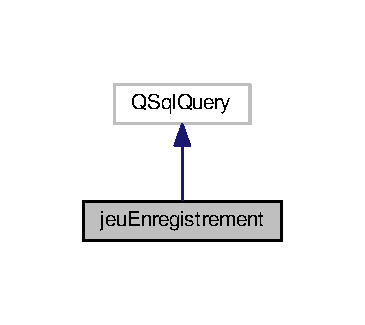
\includegraphics[width=175pt]{classjeu_enregistrement__inherit__graph}
\end{center}
\end{figure}


Collaboration diagram for jeu\+Enregistrement\+:\nopagebreak
\begin{figure}[H]
\begin{center}
\leavevmode
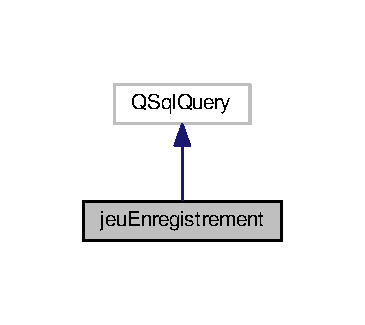
\includegraphics[width=175pt]{classjeu_enregistrement__coll__graph}
\end{center}
\end{figure}
\subsection*{Public Member Functions}
\begin{DoxyCompactItemize}
\item 
\mbox{\Hypertarget{classjeu_enregistrement_a9ea63096be94ef11f0fd08d6554aa115}\label{classjeu_enregistrement_a9ea63096be94ef11f0fd08d6554aa115}} 
{\bfseries jeu\+Enregistrement} (Q\+String chaine\+S\+QL)
\item 
\mbox{\Hypertarget{classjeu_enregistrement_aa26dd78c24b4fbaec948380d8907d4d9}\label{classjeu_enregistrement_aa26dd78c24b4fbaec948380d8907d4d9}} 
void \hyperlink{classjeu_enregistrement_aa26dd78c24b4fbaec948380d8907d4d9}{suivant} ()
\begin{DoxyCompactList}\small\item\em \hyperlink{classjeu_enregistrement_aa26dd78c24b4fbaec948380d8907d4d9}{jeu\+Enregistrement\+::suivant} Avance le curseur sur l\textquotesingle{}enregistrement suivant \end{DoxyCompactList}\item 
bool \hyperlink{classjeu_enregistrement_ad4689ab49e4a51fde86e3b00e15e473e}{fin\+Req} ()
\begin{DoxyCompactList}\small\item\em \hyperlink{classjeu_enregistrement_ad4689ab49e4a51fde86e3b00e15e473e}{jeu\+Enregistrement\+::fin\+Req} \end{DoxyCompactList}\item 
Q\+Variant \hyperlink{classjeu_enregistrement_acd8e0e1bc08d6b1a5c5966d565e134a2}{get\+Valeur} (Q\+String nom\+Champ)
\begin{DoxyCompactList}\small\item\em \hyperlink{classjeu_enregistrement_acd8e0e1bc08d6b1a5c5966d565e134a2}{jeu\+Enregistrement\+::get\+Valeur} \end{DoxyCompactList}\item 
\mbox{\Hypertarget{classjeu_enregistrement_adee0dc84769c49230dbd6b32ec0bd946}\label{classjeu_enregistrement_adee0dc84769c49230dbd6b32ec0bd946}} 
void \hyperlink{classjeu_enregistrement_adee0dc84769c49230dbd6b32ec0bd946}{fermer} ()
\begin{DoxyCompactList}\small\item\em \hyperlink{classjeu_enregistrement_adee0dc84769c49230dbd6b32ec0bd946}{jeu\+Enregistrement\+::fermer} Ferme le curseur et libère les ressources. \end{DoxyCompactList}\end{DoxyCompactItemize}


\subsection{Member Function Documentation}
\mbox{\Hypertarget{classjeu_enregistrement_ad4689ab49e4a51fde86e3b00e15e473e}\label{classjeu_enregistrement_ad4689ab49e4a51fde86e3b00e15e473e}} 
\index{jeu\+Enregistrement@{jeu\+Enregistrement}!fin\+Req@{fin\+Req}}
\index{fin\+Req@{fin\+Req}!jeu\+Enregistrement@{jeu\+Enregistrement}}
\subsubsection{\texorpdfstring{fin\+Req()}{finReq()}}
{\footnotesize\ttfamily bool jeu\+Enregistrement\+::fin\+Req (\begin{DoxyParamCaption}{ }\end{DoxyParamCaption})}



\hyperlink{classjeu_enregistrement_ad4689ab49e4a51fde86e3b00e15e473e}{jeu\+Enregistrement\+::fin\+Req} 

\begin{DoxyReturn}{Returns}
Un bool false or true si la requête est finie ou non 
\end{DoxyReturn}
\mbox{\Hypertarget{classjeu_enregistrement_acd8e0e1bc08d6b1a5c5966d565e134a2}\label{classjeu_enregistrement_acd8e0e1bc08d6b1a5c5966d565e134a2}} 
\index{jeu\+Enregistrement@{jeu\+Enregistrement}!get\+Valeur@{get\+Valeur}}
\index{get\+Valeur@{get\+Valeur}!jeu\+Enregistrement@{jeu\+Enregistrement}}
\subsubsection{\texorpdfstring{get\+Valeur()}{getValeur()}}
{\footnotesize\ttfamily Q\+Variant jeu\+Enregistrement\+::get\+Valeur (\begin{DoxyParamCaption}\item[{Q\+String}]{nom\+Champ }\end{DoxyParamCaption})}



\hyperlink{classjeu_enregistrement_acd8e0e1bc08d6b1a5c5966d565e134a2}{jeu\+Enregistrement\+::get\+Valeur} 


\begin{DoxyParams}{Parameters}
{\em nom\+Champ} & variable de S\+QL \\
\hline
\end{DoxyParams}
\begin{DoxyReturn}{Returns}
la valeur correspondant a nom\+Champ 
\end{DoxyReturn}


The documentation for this class was generated from the following files\+:\begin{DoxyCompactItemize}
\item 
/home/jeremy/\+Documents/qt\+Creator/\+Generation\+P\+D\+F\+\_\+\+Atlantik/jeuenregistrement.\+h\item 
/home/jeremy/\+Documents/qt\+Creator/\+Generation\+P\+D\+F\+\_\+\+Atlantik/jeuenregistrement.\+cpp\end{DoxyCompactItemize}

\hypertarget{class_passerelle}{}\section{Passerelle Class Reference}
\label{class_passerelle}\index{Passerelle@{Passerelle}}
\subsection*{Static Public Member Functions}
\begin{DoxyCompactItemize}
\item 
static Q\+Vector$<$ \hyperlink{class_equipement}{Equipement} $>$ \hyperlink{class_passerelle_a612df1d1532ab6a58efe8c0af66858a4}{charger\+Les\+Equipements} (Q\+String un\+Id\+Bateau)
\begin{DoxyCompactList}\small\item\em \hyperlink{class_passerelle_a612df1d1532ab6a58efe8c0af66858a4}{Passerelle\+::charger\+Les\+Equipements}. \end{DoxyCompactList}\item 
static Q\+Vector$<$ \hyperlink{class_bateau_voyageur}{Bateau\+Voyageur} $>$ \hyperlink{class_passerelle_a9f8cdd9d52d668bb33a5380324fb9c51}{charger\+Les\+Bateaux\+Voyageurs} ()
\begin{DoxyCompactList}\small\item\em \hyperlink{class_passerelle_a9f8cdd9d52d668bb33a5380324fb9c51}{Passerelle\+::charger\+Les\+Bateaux\+Voyageurs}. \end{DoxyCompactList}\end{DoxyCompactItemize}


\subsection{Member Function Documentation}
\mbox{\Hypertarget{class_passerelle_a9f8cdd9d52d668bb33a5380324fb9c51}\label{class_passerelle_a9f8cdd9d52d668bb33a5380324fb9c51}} 
\index{Passerelle@{Passerelle}!charger\+Les\+Bateaux\+Voyageurs@{charger\+Les\+Bateaux\+Voyageurs}}
\index{charger\+Les\+Bateaux\+Voyageurs@{charger\+Les\+Bateaux\+Voyageurs}!Passerelle@{Passerelle}}
\subsubsection{\texorpdfstring{charger\+Les\+Bateaux\+Voyageurs()}{chargerLesBateauxVoyageurs()}}
{\footnotesize\ttfamily Q\+Vector$<$ \hyperlink{class_bateau_voyageur}{Bateau\+Voyageur} $>$ Passerelle\+::charger\+Les\+Bateaux\+Voyageurs (\begin{DoxyParamCaption}{ }\end{DoxyParamCaption})\hspace{0.3cm}{\ttfamily [static]}}



\hyperlink{class_passerelle_a9f8cdd9d52d668bb33a5380324fb9c51}{Passerelle\+::charger\+Les\+Bateaux\+Voyageurs}. 

\begin{DoxyReturn}{Returns}
un vecteur des infos du bateau S\textquotesingle{}apprête a renvoyer un vector On récupère toutes les information concernant tout les bateaux voyageurs 
\end{DoxyReturn}
\mbox{\Hypertarget{class_passerelle_a612df1d1532ab6a58efe8c0af66858a4}\label{class_passerelle_a612df1d1532ab6a58efe8c0af66858a4}} 
\index{Passerelle@{Passerelle}!charger\+Les\+Equipements@{charger\+Les\+Equipements}}
\index{charger\+Les\+Equipements@{charger\+Les\+Equipements}!Passerelle@{Passerelle}}
\subsubsection{\texorpdfstring{charger\+Les\+Equipements()}{chargerLesEquipements()}}
{\footnotesize\ttfamily Q\+Vector$<$ \hyperlink{class_equipement}{Equipement} $>$ Passerelle\+::charger\+Les\+Equipements (\begin{DoxyParamCaption}\item[{Q\+String}]{un\+Id\+Bateau }\end{DoxyParamCaption})\hspace{0.3cm}{\ttfamily [static]}}



\hyperlink{class_passerelle_a612df1d1532ab6a58efe8c0af66858a4}{Passerelle\+::charger\+Les\+Equipements}. 


\begin{DoxyParams}{Parameters}
{\em un\+Id\+Bateau} & \+: Identifie le bateau \\
\hline
\end{DoxyParams}
\begin{DoxyReturn}{Returns}
les equipements du bateau S\textquotesingle{}apprête a renvoyer un vector Récuperer les equipements en fonction du bateau séléctionné 
\end{DoxyReturn}


The documentation for this class was generated from the following files\+:\begin{DoxyCompactItemize}
\item 
/home/jeremy/\+Documents/qt\+Creator/\+Generation\+P\+D\+F\+\_\+\+Atlantik/passerelle.\+h\item 
/home/jeremy/\+Documents/qt\+Creator/\+Generation\+P\+D\+F\+\_\+\+Atlantik/passerelle.\+cpp\end{DoxyCompactItemize}

\hypertarget{class_p_d_f}{}\section{P\+DF Class Reference}
\label{class_p_d_f}\index{P\+DF@{P\+DF}}


Inheritance diagram for P\+DF\+:\nopagebreak
\begin{figure}[H]
\begin{center}
\leavevmode
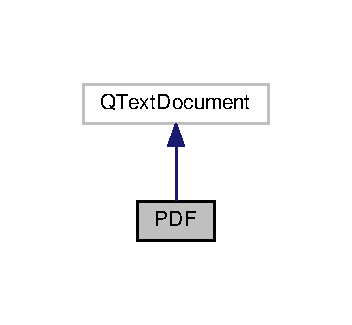
\includegraphics[width=169pt]{class_p_d_f__inherit__graph}
\end{center}
\end{figure}


Collaboration diagram for P\+DF\+:\nopagebreak
\begin{figure}[H]
\begin{center}
\leavevmode
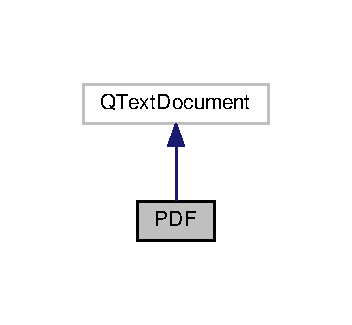
\includegraphics[width=169pt]{class_p_d_f__coll__graph}
\end{center}
\end{figure}
\subsection*{Public Member Functions}
\begin{DoxyCompactItemize}
\item 
\mbox{\Hypertarget{class_p_d_f_a67ddabfeb5a32f6fe6517778dc0f619c}\label{class_p_d_f_a67ddabfeb5a32f6fe6517778dc0f619c}} 
{\bfseries P\+DF} (Q\+String nom\+Document)
\item 
void \hyperlink{class_p_d_f_a7bb38923f4141702b3772ec41213917f}{ecrire\+Texte} (Q\+String le\+Texte)
\begin{DoxyCompactList}\small\item\em \hyperlink{class_p_d_f_a7bb38923f4141702b3772ec41213917f}{P\+D\+F\+::ecrire\+Texte}. \end{DoxyCompactList}\item 
void \hyperlink{class_p_d_f_a3c7d97ad7f3c7a390272d05c7f95e832}{charger\+Image} (Q\+String chemin)
\begin{DoxyCompactList}\small\item\em \hyperlink{class_p_d_f_a3c7d97ad7f3c7a390272d05c7f95e832}{P\+D\+F\+::charger\+Image}. \end{DoxyCompactList}\item 
\mbox{\Hypertarget{class_p_d_f_a96a1cc767274d19eedec45ff7aca6b7a}\label{class_p_d_f_a96a1cc767274d19eedec45ff7aca6b7a}} 
void \hyperlink{class_p_d_f_a96a1cc767274d19eedec45ff7aca6b7a}{fermer} ()
\begin{DoxyCompactList}\small\item\em \hyperlink{class_p_d_f_a96a1cc767274d19eedec45ff7aca6b7a}{P\+D\+F\+::fermer} On enregistre via print en faisant passer l\textquotesingle{}imprimante en conversion de pdf. \end{DoxyCompactList}\end{DoxyCompactItemize}


\subsection{Member Function Documentation}
\mbox{\Hypertarget{class_p_d_f_a3c7d97ad7f3c7a390272d05c7f95e832}\label{class_p_d_f_a3c7d97ad7f3c7a390272d05c7f95e832}} 
\index{P\+DF@{P\+DF}!charger\+Image@{charger\+Image}}
\index{charger\+Image@{charger\+Image}!P\+DF@{P\+DF}}
\subsubsection{\texorpdfstring{charger\+Image()}{chargerImage()}}
{\footnotesize\ttfamily void P\+D\+F\+::charger\+Image (\begin{DoxyParamCaption}\item[{Q\+String}]{chemin }\end{DoxyParamCaption})}



\hyperlink{class_p_d_f_a3c7d97ad7f3c7a390272d05c7f95e832}{P\+D\+F\+::charger\+Image}. 


\begin{DoxyParams}{Parameters}
{\em chemin} & \+: Chemin d\textquotesingle{}ou se trouve l\textquotesingle{}image \\
\hline
\end{DoxyParams}
\mbox{\Hypertarget{class_p_d_f_a7bb38923f4141702b3772ec41213917f}\label{class_p_d_f_a7bb38923f4141702b3772ec41213917f}} 
\index{P\+DF@{P\+DF}!ecrire\+Texte@{ecrire\+Texte}}
\index{ecrire\+Texte@{ecrire\+Texte}!P\+DF@{P\+DF}}
\subsubsection{\texorpdfstring{ecrire\+Texte()}{ecrireTexte()}}
{\footnotesize\ttfamily void P\+D\+F\+::ecrire\+Texte (\begin{DoxyParamCaption}\item[{Q\+String}]{le\+Texte }\end{DoxyParamCaption})}



\hyperlink{class_p_d_f_a7bb38923f4141702b3772ec41213917f}{P\+D\+F\+::ecrire\+Texte}. 


\begin{DoxyParams}{Parameters}
{\em le\+Texte} & \+: Correspond à la chaîne avec toutes les infos Je récupère vers\+Chaine(chaine\+A\+Retourner) qui est dans bateau\+Voyageur.\+cpp \\
\hline
\end{DoxyParams}


The documentation for this class was generated from the following files\+:\begin{DoxyCompactItemize}
\item 
/home/jeremy/\+Documents/qt\+Creator/\+Generation\+P\+D\+F\+\_\+\+Atlantik/pdf.\+h\item 
/home/jeremy/\+Documents/qt\+Creator/\+Generation\+P\+D\+F\+\_\+\+Atlantik/pdf.\+cpp\end{DoxyCompactItemize}

%--- End generated contents ---

% Index
\backmatter
\newpage
\phantomsection
\clearemptydoublepage
\addcontentsline{toc}{chapter}{Index}
\printindex

\end{document}
